\section{Related work}
\label{introduction-related-work}
% Related work summary, only stuff that's directly relevant for our research. Other references can be made later by simply mentioning them. Avoid summarizing related work in too much detail, keep it clear and concise. We need to show our contribution, not what others did.
% short intro about this section needed, connecting the pid and ndn part

In this section we will provide an overview of existing solutions for \gls{pid} interoperability and known \gls{ndn} performance and scalability issues and solutions.

\subsection{PID interoperability}
\label{introduction-pid}
In 2014, Karakannas researched the efficiency of \gls{icn} for delivering big data with \glspl{pid} \cite{icn-bd}. \glspl{pid} are used in big data infrastructures to identify digital content and research data. The research proposed a mapping architecture for resolving \glspl{pid} to \gls{icn} names. Karakannas proposed to use a \gls{pid} to \gls{ndn} mapping server for every \gls{pid} type instead of implementing the translation on the clients browser. For the latter, the researcher states that translation of a \gls{pid} to \gls{ndn} name will be highly depended on the clients \gls{ndn} browser, which needs to be updated every time a new \gls{pid} schema would be introduced \cite{icn-bd}.
%The research results showed that in-network caching can offer significant performance benefits, when the cache size of the network elements that perform in-network caching is bigger than the Big Data object size. 

In 2017, Mousa researched the fetching and sharing of \gls{doi} objects with \gls{icn} such as \gls{ndn}. 
The researcher's approach focused only on \gls{doi} identified objects within \gls{ndn}'s, which was possible. Mousa stated that there are many other different \gls{pid} systems that can also be identified and translated for compatibility with the \gls{ndn} naming schema. The patterns of most of these different \gls{pid} systems are maintained in the ePIC \gls{dtr} \cite{dtr}.
 Furthermore, the researcher explained that the difference in \gls{ndn} naming of different \gls{pid} providers must be taken into account, such that the correct prefix is used within \gls{ndn} to identify specific \gls{pid} types. For example, using the prefix \texttt{"doi/"} within \gls{ndn} for \gls{doi} identified objects.
In the researcher's design, the translation happens in the consumers browsers. The consumer has the choice to either request the digital object by its \gls{ndn} name or \gls{pid} \cite{ndn-app-aware}.

Zhao et al. progressed the research done by Karakannas \cite{icn-bd} and Mousa \cite{ndn-app-aware} and proposed an architecture to map \glspl{pid} into the naming schema of \gls{ndn}. Their proposed solution is called \gls{naas4pid} and supports one \gls{pid} type. This solution is composed out of three key components \cite{koulouzis2018information}:
\begin{itemize}
  \item \gls{pid}2\gls{ndn} gateway; primarily responsible for resolving \glspl{pid} to \gls{ndn} names.
  \item \gls{ndn}4\gls{pid} router image; an \gls{ndn} node that implements a virtualized \gls{ndn} router.
  \item \gls{ndn}4\gls{pid} manager; automates the management of the \gls{ndn} overlay in\newline cloud or e-infrastructure.
\end{itemize}

Olschanowsky et. al. researched translating climate modeling schema filenames, used by \gls{cmmap} applications at Colorado State University, to an \gls{ndn} compatible 
naming schema. The researchers designed an \gls{ndn} name translator to support the data management needs of \gls{cmmap}. The \gls{ndn} name translator incorporates a naming schema that is designed to be compatible with existing climate modeling schemas, like the \gls{cmip}. While allowing for some flexibility for project-specific requirements. They explained that \gls{ndn} names for climate data should be both expressive and human readable. The advantages of long expressive names versus short easy to remember names have to be balanced.
The researchers stated that every data provider should publish a data prefix which acts as a globally
routable prefix within \gls{ndn} covering all of the data made available by the provider. This complies with Mousa, who stated that \gls{ndn} naming of different \gls{pid} providers must be taken into account. The researchers consulted with \gls{cmmap} climate scientists and confirmed that these naming rules are acceptable for their data sets and are appropriate for global distribution. 
However, the translation is not as simple as taking only the filename and translate it into an \gls{ndn} name. To construct appropriate \gls{ndn} names to uniquely identify data of a specific model, the filename to \gls{ndn} translator needs information gleaned from the filesystem path, filename and metadata mined from the data itself. This information is processed by a filename to \gls{ndn} name mapping schema to use it for \gls{cmmap} filenames. Therefore, some intelligence is expected in their translators.
Figure \ref{fig:cmmap_ndnn}, taken from Olschanowsky et. al., shows the translation of a \gls{cmmap} to an \gls{ndn} name. In this example it is shown that after the prefix \texttt{"/coupled/control/CMMAP/"}, which identifies the provider, the \gls{ndn} translated name contains additional information next to the input filename \cite{ndn-clim}.
%, which is parsed from metadata or information that resides in the data itself \cite{ndn-clim}. 
They further stated that since \gls{ndn} naming is flexible and virtually any appropriate translation schema can be plugged into, it is possible to support many naming schemas as long as the name can be broken down in hierarchical components.

\begin{figure}[H]
\centering
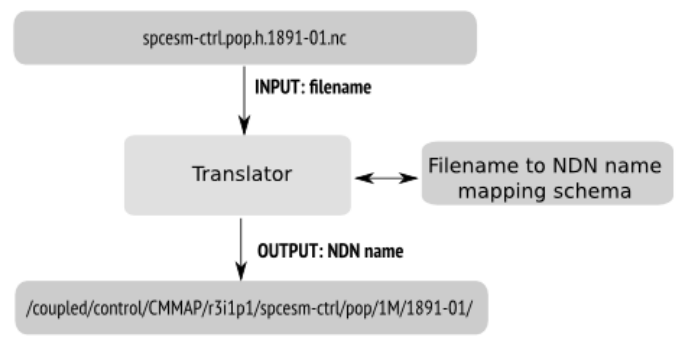
\includegraphics[scale=0.4]{Images/cmip2ndn.png}
\caption{CMMAP to \gls{ndn} name translator.}
\label{fig:cmmap_ndnn}
\end{figure}

The research done by Fan et. al. utilizes a catalog which contains the translation of \gls{ndn} names. Users query the catalogue to receive an \gls{ndn} name. This process is fairly lightweight since the catalog's only concern is to add or remove names rather than data set synchronization. The researchers used data sets of the \gls{cmip} climate modeling schema for their research and encourage to use the climate modeling schema as a prefix for an \gls{ndn} name. This is comparable and also complies with the previous researches, where \gls{ndn} naming of different \gls{pid} providers must be taken into account.
Their catalog design can support the needs of any community, which can be seen as a data provider described earlier. The catalog is able to define and use consistent naming schemas.
The researchers concluded that their catalog facilitates \gls{ndn} name discovery and that data management can be made easier for scientific communities as long as they converge on common naming schemas \cite{ndn-man}. 

\subsection{NDN performance and scalability}
\label{introduction-related-work-ndn}
ICN is the common architectural idea of forwarding packets based on their name rather than destination (IP) \cite{jacobson2009networking}. Research done by Karakannas \cite{icn-bd} concluded that \gls{ndn} was the only \gls{icn} approach that published a specification and workable software to experiment with. As of writing this report, we concluded that this conclusion is still valid. Therefore, this research used \gls{ndn} for experimentation. The reasoning behind the choice for \gls{ndn} compared to other solutions is discussed in more detail in section \ref{introduction-ndn}.

James McCabe's "Network Analysis, Architecture, and Design" \cite{mccabe2010network} book offers a systems methodology approach towards network design. The approach is described in McCabe as "seeing the network part of a larger system, with interactions and dependencies between the network and its users, applications and devices". The methodology put forward by McCabe is to design a network based on several inputs and outputs:
\begin{itemize}
    \item Analysis: What do users/services require? How are the relationships composed between these components?
    \item Architecture: Which technology and topology choices support the users/services needs? Based on this, create high-level, end-to-end structure of the network.
    \item Design: Determine the physical detail of the architecture based on output of the previous steps.
\end{itemize}

% The inputs and outputs used in this method are intended to be iterative and by no means define a final architectural design. This is due to the fact that requirements, technology and user behavior can change and with that the network design. 

Section \ref{overview-mccabe} provides a more detailed overview of this method and section \ref{planning-ndn} describes how it is applied for this research.

NDN is not yet implemented on a large scale, with the exception of several large testbeds. In order to plan an \gls{ndn}, it would be necessary to know what works and does not work. However, there is sufficient research available that focused on particular design choices of \gls{ndn}. Research done by Lim et al. \cite{lim2018ndn} at a large existing testbed located in the USA \cite{ndn-testbed-status} highlighted a few lessons learned. Lim et al. setup the first intercontinental \gls{ndn} testbed with the intent to see the benefits for big science. They implemented a name translator for climate-science data, which translated \gls{cmip} files to an \gls{ndn} compatible name. They concluded that \gls{ndn} provided performance improvements compared to classical climate data delivery techniques based on TCP/IP. An experimental network between universities was used for testing which provided direct links across the USA. The research concluded that \gls{ndn} over UDP does not properly support large \gls{ndn} packets (\textgreater 64kB). According to the research this was due to UDP's properties of not applying congestion control and proper packet retransmission and resulted in unsatisfying performance. The loss of a single UDP segment resulted in the retransmission of a large \gls{ndn} data packet, consisting out of many UDP packets. However, they did not consider the lack of flow and congestion control in the \gls{ndn} software. The researchers also didn't take into account the theoretical limit of UDP packets which with the IPv4 protocol is 65,507 bytes (65,535 - 8 byte UDP header - 20 byte IP header), thus fragmentation is expected. Furthermore, \gls{ndn} over TCP demonstrated a more reliable and faster performance due to the allowance of larger dynamic window sizes and congestion control. Native \gls{ndn} congestion control is still an open research area \cite{ren2016congestion}, as of writing this report, no proposal has been implemented.

The performance benefits of \gls{ndn} concluded by Lim et al. correlates with research done by Shannigrahi et al. at the USA-based large hadron collider network \cite{shannigrahi2015named}. The researchers achieved a 71\% reduction in the average delay per data chunk compared to a no-caching case. They conducted \gls{ndn} caching simulations \cite{shannigrahi2017request}, where they concluded that a small cache of several gigabytes already reduces the network load. However, as expected, increasing the cache towards 1TB reduced the network load even further. However, this reduction of load wasn't proportional to the cache size. They concluded in their research that a 1GB \gls{ndn} cache at the edge of the \gls{ndn} can already significantly improve data distribution and reduce the network load. The average file size in use was 1.3GB.

Furthermore, in \gls{ndn} several caching, cache replacement and forwarding strategies can be used to fine-tune performance. Koulouzis et al. researched these strategies and concluded that the 'leave copy everywhere' caching strategy provided the best performance ratio between cache size to data object size for generic data usage. However, 'leave copy down' and 'leaving copies with probability' performed best for delivering big data objects. Koulouzis et al. also concluded that the ascending ordering of data objects enhances network performance when combined with the 'least recently used' caching strategy. This was concluded based on observations that if large objects were requested first, the cache replacement algorithm would make room by overwriting files already in the cache, resulting in cache misses. When small files were requested first, more cache hits were measured. As for cache size, the researchers recommended a cache size at least twice the size of the biggest data object in the network \cite{koulouzis2018information}.

Yuan et al. \cite{yuan2012scalable} researched the performance of \gls{ndn} forwarding. They used the \gls{ccnx} application\footnote{\url{https://wiki.fd.io/view/Cicn}} to perform experiments. Their research concluded that packets with long names degraded performance. After profiling the software they measured that the \gls{ndn} name decode operation took 35.46\% of the entire program running time. So et al. \cite{so2013named} developed a method to achieve fixed lookup times with variable length names. In order to achieve this goal they explored the application of hash tables to do name lookup. Furthermore, they explored the possibility to do this in hardware by using a Cisco ASR9000 router with the integrated service module running 64-bit Linux. With their experiments they managed to forward 20Gbps of real \gls{ndn} traffic. Tortelli et al. \cite{tortelli2013performance} researched the effectiveness of two opposite forward strategies; flooding and best-route (with and without caching). Several experiments lead them to the conclusion that there are pros and cons in each forwarding strategy. But that it is difficult to determine the best performing forward strategy.

The heterogeneous nature in cloud environments can make deployment automation and management complicated. \gls{tosca} \cite{tosca-standard} is a method to describe the deployment and management of a cloud infrastructure based on reusable templates. These descriptions are then used by orchestrators to facilitate the deployment. SeaClouds \cite{seaclouds-website} (\gls{fp7} funded project), not to be confused with SeaDataCloud, is a research cloud that already manages infrastructures based on TOSCA. Brogi et al. \cite{brogi2015adaptive} concluded that SeaClouds can now realize their multiple cloud infrastructures in an automated arrangement with central coordination, deployment and management without the need to make custom deployment strategies for each cloud environment. Furthermore, several large companies such as Google, Red Hat, Canonical and IBM are also involved with the development of TOSCA, signifying that broader adoption may follow in the future.

% deze zin is te complex, zonder te weten hoe ndn werkt, dat komt later meer aan bod
%The \gls{ndn} router that has cached the \gls{ndn} objects acts as a producer. The client which retrieves the object acts as a client in our setup. 

%This design is implemented in the second methodology section,
%which includes showing our proposed design that describes how \gls{pid} interoperability in the \gls{ndn} namespace can be achieved. 

%Furthermore, this section will bring the attention of how to plan a \gls{ndn} network by using orchestration tools such as McCabe
%and \gls{tosca} 
%and how \gls{ndn} scalability is achieved. 
%After the aforementioned section we will get to the results in section \ref{res} to show the results we got from the experiments based on our methodology.


%then follows in section \ref{disc} where we discuss our proposed solution 

%to discuss difficulties we came across during our research and what advice can be given to the reader.
 

% To guide the reader into what's to come, can be done only when whole report is done